\documentclass{article}
\usepackage[UTF8]{ctex} % 用于中文排版
\usepackage{geometry}
\usepackage{indentfirst}
\usepackage{enumitem}

\usepackage{titling}    % 用于自定义标题页
\usepackage{graphicx}
\usepackage{float}

\usepackage{xcolor}
\usepackage{listings}

\usepackage{setspace}

% 页面几何设置
\geometry{a4paper, left=25mm, right=25mm, top=25mm, bottom=25mm}
% 取消首行缩进
\setlength{\parindent}{0pt}
% 行间距设置
\setstretch{1.5}
% 自定义字体大小
\newcommand{\fourhao}{\fontsize{14pt}{\baselineskip}\selectfont} % 四号字体
\newcommand{\xiaosihao}{\fontsize{12pt}{\baselineskip}\selectfont} % 小四号字体
\newcommand{\song}{\CJKfamily{song}}
% 设置代码块格式
\lstset{
    basicstyle = \footnotesize\ttfamily,                 % 设置行距,字体
    numbers = left,                                      % 在左侧显示行号
    numberstyle = \tiny \color{gray},                    % 设定行号格式
    keywordstyle = \bfseries \color[RGB]{40,40,255},     % 设定关键字颜色
    numberstyle = \footnotesize \color{darkgray},           
    commentstyle = \color[RGB]{0,96,96},                 % 设置代码注释的格式
    stringstyle = \color[RGB]{128,0,0},                  % 设置字符串格式
    frame = single,                                      % 不显示背景边框
    backgroundcolor = \color[RGB]{245,245,244},          % 设定背景颜色
    language=Verilog                                     % 设置语言
}
\raggedbottom   % 段落间留白, 避免排版时自动拉伸导致的行间距变化。
\begin{document}

% 封面页面
\begin{titlepage}
    \centering
    \vspace*{2cm}

    \Huge
    \textbf{课程名称:EDA 技术综合设计}

    \vspace{2cm}

    \LARGE
    设计报告名称:设计五\ 交通灯控制器

    \vspace{4cm}

    \centering
    \Large
    \begin{tabular}{rl}
        班级: & 通信214    \\
        姓名: & \ 王峤宇    \\
        学号: & \ 214022
    \end{tabular}

    \vfill

    \vspace{1cm}
\end{titlepage}

\newpage
% 第一部分
\section*{\fourhao 一、设计内容及原理}
\xiaosihao
\setstretch{1.5}
% 设计项目内容及设计原理,如真值表、状态表及状态转换图、文字说明等。
\subsection*{基础任务}
\textbf{设计任务}:十字路口东西、南北各有红、黄、绿指示灯,其中绿 灯、黄灯和红灯的持续时间分别为 40s、5s 和 45s。 状态机所包含的
状态有四个(S0,S1,S2,S3)如下:\\
S0:东西绿灯亮,红灯和黄灯灭;南北绿灯和黄灯灭,红灯亮。\\
S1:东西绿灯和红灯灭,黄灯亮;南北绿灯和黄灯灭,红灯亮。\\
S2:东西绿灯和黄灯灭,红灯亮;南北绿灯亮,红灯和黄灯灭。\\
S3:东西绿灯和黄灯灭,红灯亮;南北绿灯和红灯灭,黄灯亮。\\
其中 S0、S2 状态应该持续 40 秒,S1、S3 状态应该持续 5 秒。
该功 能采用计数器计时实现,由一个辅助进程来完成,包含一个最大计数值为 39 的计数器和一个最大计数值为 4 的计数器。
计数器的使能控制根据当前状态决定,计数器的进位位输出作为状态机的控制输入。东西、南北红、绿、黄灯点亮由状态机的输出控制。
由数码管显示输出当前路口两个方向当前灯的剩余时间。\\

\subsubsection*{状态机}
状态机分为Moore型和Mealy型状态机, Moore型状态机的输出由仅有当前状态决定, 而Mealy型状态机的输出与当前状态和当前输入有关。\\
状态机一般指有限状态机(FSM), 表示系统中的有限个状态以及这些状态间的转移和动作的模型。\\
Verilog中的状态机有一段式描述风格、两段式描述风格以及三段式描述风格, 通常主要使用三段式描述风格, 通过三个always块描述一个状态机:状态切换用的时序逻辑电路、次态输出的组合逻辑、信号输出用的时序逻辑。
两段式FSM与三段式的区别主要是, 其信号输出由组合逻辑负责。三段式描述风格可以使FSM做到了同步寄存器输出,
消除了组合逻辑输出的不稳定与毛刺的隐患,因此本次设计采用三段式描述风格。\\
\begin{figure}[htbp]
    \centering
    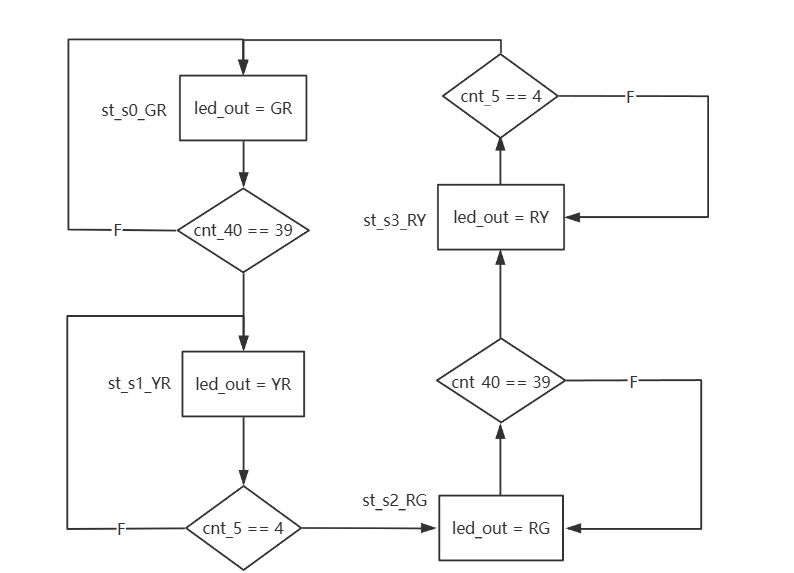
\includegraphics[width=0.5\textwidth]{image/2024-06-19-10-48-41.png}
    \caption{基础任务ASM图}
    \label{image_asm_1}
\end{figure}
基础任务设计的状态机的ASM有限状态机描述如图\ref{image_asm_1}所示:
\subsection*{提高内容}
\textbf{设计任务}:在基础任务的基础上,加一个检修状态(由检修信号控制),从任何 状态都可以进入检修状态,检修时间不定,但是检修结束后延迟 5 秒进入 S0 状态。\\
实现检修状态, 添加两个状态, 一个是检修状态, 一个检修退出状态。
\begin{figure}[htbp]
    \centering
    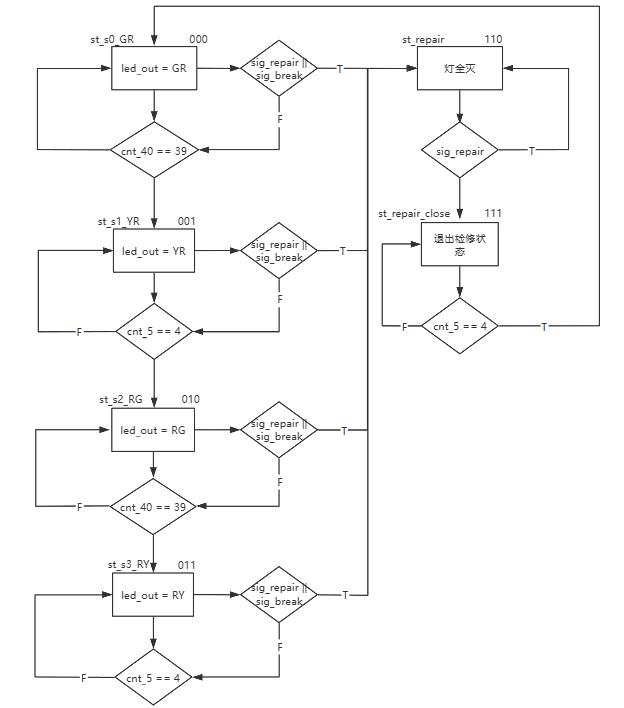
\includegraphics[width=0.7\textwidth]{image/2024-06-19-14-38-12.png}
    \caption{检修状态ASM图}
    \label{image_asm_2}
\end{figure}
该任务的ASM图如图\ref{image_asm_2}所示, 在求解次态输出时, 需要对输入的检修信号进行监听。
\subsection*{拓展任务}
\textbf{任务要求}:在拓展任务的基础上,东西南北方向都加入附加状态, 由按键或拨码开关控制(给出信号后收回,及按键触发后松开,
拨码 开关拨上后紧接着拨下,算是触发一次),不管当前是什么状态,只 要东西或者南北方向有附加按键触发,再当前状态结束后,都不
转移 到下一个状态,而是所有状态暂停 30 秒,30 秒后自动恢复进入下一个即将进入的状态(实际上是加上了行人过马路的触发状态)\\

实现附加状态的关键点在于, 其相当于在任意两个相邻转移状态间插入一个状态, 针对该中断触发式的状态, 由于每次进出附加状态的状
态都不同, 但种类并不多, 所以采用多个附加状态的形式实现。\\
\begin{figure}[htbp]
    \centering
    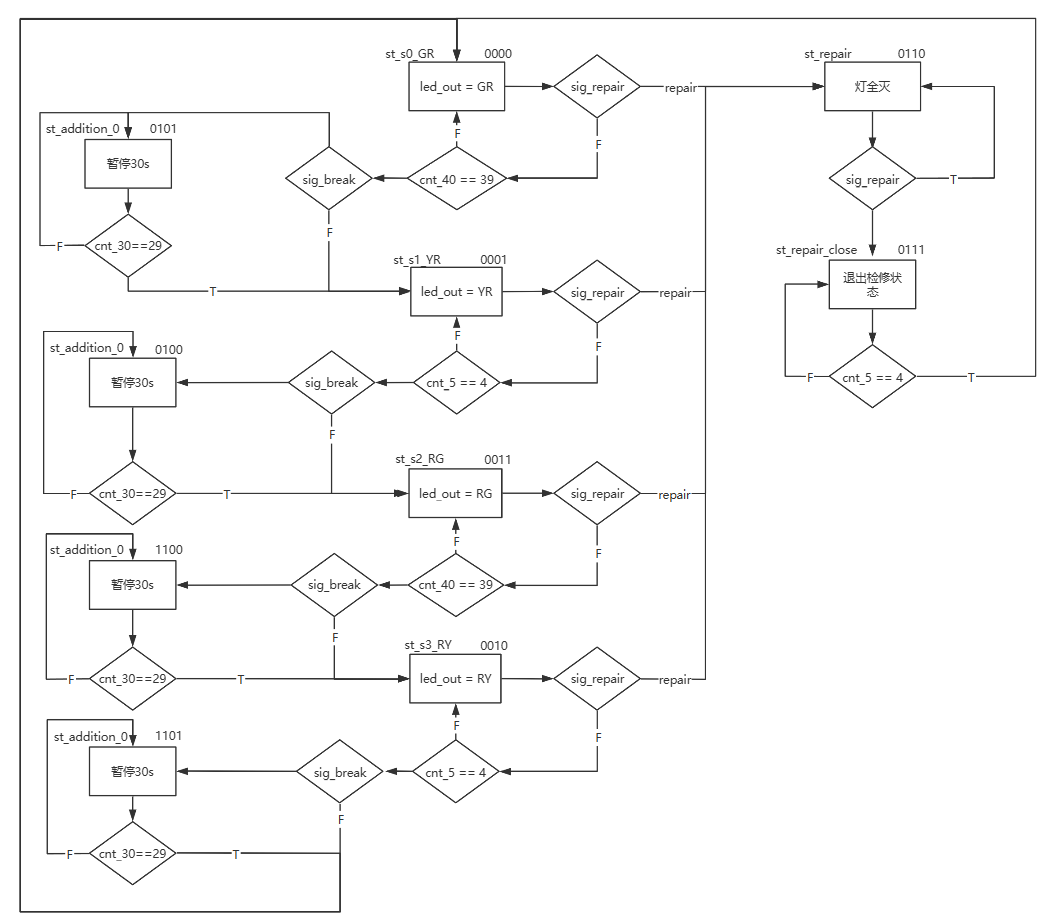
\includegraphics[width=0.7\textwidth]{image/2024-06-19-18-06-00.png}
    \caption{附加状态ASM图}
    \label{image_asm_3}
\end{figure}
实现附加状态后的ASM图见\ref{image_asm_3}
% 第二部分
\section*{\fourhao 二、设计过程}
\xiaosihao
\setstretch{1.5}
% 从工程建立开始,一直到硬件调试。
% 按照基础任务、提高任务和拓展任务分别给出相应的源文件、仿真文件、约束文件
\subsection*{基础任务}
交通灯控制基础任务的源文件如下:
\begin{lstlisting}[language=Verilog, caption={交通灯控制基础任务源文件}]
// `define STIMULATION

module traffic_light(
    input sys_clk,                      /* 系统100MHz时钟 */
    input rst,                          /* 高电平, 异步复位 */
    input sig_repair,                   /* 检修状态信号, 高电平有效 */
    input sig_break,                    /* 30s的附加状态信号, 上升沿有效 */
    output reg [2:0] led_east_west,     /* 东西方向红-黄-绿灯 */
    output reg [2:0] led_north_south,   /* 南北方向红-黄-绿灯 */
    output [7:0] sseg1, sseg2,          /* 八段数码管 */
    output [3:0] an1, an2               /* 数码管片选信号 */
    );
    
    `ifdef STIMULATION
    assign clk_1Hz = sys_clk;
    `else
    wire clk_1Hz;
    /* 产生1.00117Hz信号 */
    clk_div_32bit  clk_div_32bit_inst (
        .clk(sys_clk),
        .rstn(!rst),
        .step_freq(32'd43),
        .clk_out(clk_1Hz)
    );
    `endif

    // 交通灯控制器一共有7个状态, 使用格雷码指定状态
    localparam st_s0_GR = 3'b000;       /* 东西绿灯亮, 南北红灯亮, 40s */
    localparam st_s1_YR = 3'b001;       /* 东西黄灯亮, 南北红灯亮, 5s */
    localparam st_s2_RG = 3'b011;       /* 东西红灯亮, 南北绿灯亮, 40s */
    localparam st_s3_RY = 3'b010;       /* 东西红灯亮, 南北黄灯亮, 5s */

    localparam st_repair = 3'b110;      /* 检修进行状态 */
    localparam st_repair_close = 3'b111;/* 检修退出状态 */
    localparam st_addition = 3'b101;    /* 附加状态 */

    /* 状态转换 */
    reg [2:0] st_cur, st_nxt;
    always @(posedge clk_1Hz, posedge rst) begin
        if (rst) begin
            st_cur <= st_s0_GR;
        end
        else begin
            st_cur <= st_nxt;
        end
    end

    /* 40s定时器 */
    reg [5:0] cnt_40;
    always @(posedge clk_1Hz) begin
        if (st_cur == st_s0_GR || st_cur == st_s2_RG) begin
            cnt_40 <= cnt_40 + 1'b1;
        end
        else begin
            cnt_40 <= 6'b0;
        end
    end

    /* 5s定时器 */
    reg [2:0] cnt_5;
    always @(posedge clk_1Hz) begin
        if (st_cur == st_s1_YR || st_cur == st_s3_RY) begin
            cnt_5 <= cnt_5 + 1'b1;
        end
        else begin
            cnt_5 <= 3'b0;
        end
    end

    /* 组合逻辑次态输出 */
    always @(*) begin
        case (st_cur)
            st_s0_GR: begin
                if (cnt_40 == 6'd39) begin
                    st_nxt <= st_s1_YR;
                end
                else begin
                    st_nxt <= st_s0_GR;
                end
            end
            st_s1_YR: begin
                if (cnt_5 == 6'd4) begin
                    st_nxt <= st_s2_RG;
                end
                else begin
                    st_nxt <= st_s1_YR;
                end
            end
            st_s2_RG: begin
                if (cnt_40 == 6'd39) begin
                    st_nxt <= st_s3_RY;
                end
                else begin
                    st_nxt <= st_s2_RG;
                end
            end
            st_s3_RY: begin
                if (cnt_5 == 6'd4) begin
                    st_nxt <= st_s0_GR;
                end
                else begin
                    st_nxt <= st_s3_RY;
                end
            end
            default: st_nxt <= st_s0_GR;
        endcase
    end
    /* 时序逻辑输出, 东西方向的交通灯 */
    always @(posedge clk_1Hz) begin
        case (st_nxt)
            st_s0_GR: begin
                led_east_west <= 3'b001;
            end
            st_s1_YR: begin
                led_east_west <= 3'b010;
            end
            st_s2_RG: begin
                led_east_west <= 3'b100;
            end
            st_s3_RY: begin
                led_east_west <= 3'b100;
            end
            default: led_east_west <= 3'b000;
        endcase
    end
    /* 时序逻辑输出, 南北方向的交通灯 */
    always @(posedge clk_1Hz) begin
        case (st_nxt)
            st_s0_GR: begin
                led_north_south <= 3'b100;
            end
            st_s1_YR: begin
                led_north_south <= 3'b100;
            end
            st_s2_RG: begin
                led_north_south <= 3'b001;
            end
            st_s3_RY: begin
                led_north_south <= 3'b010;
            end
            default: led_north_south <= 3'b000;
        endcase
    end
    /* 东西方向的倒计时计算 */
    reg [5:0] countdown_1; 
    always @(*) begin
        case (st_cur)
            st_s0_GR: countdown_1 <= 6'd40 - cnt_40;
            st_s1_YR: countdown_1 <= 6'd5 - {3'b0, cnt_5};
            st_s2_RG: countdown_1 <= 6'd45 - cnt_40;
            st_s3_RY: countdown_1 <= 6'd5 - {3'b0, cnt_5};
            default: countdown_1 <= 6'b0;
        endcase
    end
    /* 南北方向的倒计时计算 */
    reg [5:0] countdown_2;
    always @(*) begin
        case (st_cur)
            st_s0_GR: countdown_2 <= 6'd45 - cnt_40;
            st_s1_YR: countdown_2 <= 6'd5 - {3'b0, cnt_5};
            st_s2_RG: countdown_2 <= 6'd40 - cnt_40;
            st_s3_RY: countdown_2 <= 6'd5 - {3'b0, cnt_5};
            default: countdown_2 <= 6'b0;
        endcase
    end
    /* 东西方向倒计时转BCD码 */
    wire [3:0] bcd_buffer_1[0:1];    /* 东西方向显示缓存 */
    bin2bcd_8bit  bin2bcd_8bit_inst_1 (
        .bin({2'b0, countdown_1}),
        .bcd_12bit({bcd_buffer_1[0], bcd_buffer_1[1]})
    );
    /* 南北方向倒计时转BCD码 */
    wire [3:0] bcd_buffer_2[0:1];    /* 南北方向显示缓存 */
    bin2bcd_8bit  bin2bcd_8bit_inst_2 (
        .bin({2'b0, countdown_2}),
        .bcd_12bit({bcd_buffer_2[0], bcd_buffer_2[1]})
    );
    /* 第一个四位数码管 */
    scan_led_hex_disp_4  scan_led_hex_disp_4_inst_1 (
        .clk(sys_clk), .rst(rst),
        .hex0(bcd_buffer_1[0]), .hex1(bcd_buffer_1[1]), .hex2(4'd10), .hex3(4'd10), .dp(4'b0000),
        .an(an1), .sseg(sseg1)
    );
    /* 第二个四位数码管 */
    scan_led_hex_disp_4  scan_led_hex_disp_4_inst_2 (
        .clk(sys_clk), .rst(rst),
        .hex0(4'd10), .hex1(4'd10), .hex2(bcd_buffer_2[0]), .hex3(bcd_buffer_2[1]), .dp(4'b0000),
        .an(an2), .sseg(sseg2)
    );
endmodule    
\end{lstlisting}
数码管源文件如下:
\begin{lstlisting}[language=Verilog, caption={数码管源文件}]
module scan_led_hex_disp_4(
    input clk, rst,
    input [3:0] hex0, hex1, hex2, hex3, /* 显存 */
    input [3:0] dp,
    output reg [3:0] an,
    output reg [7:0] sseg
    );

    localparam N = 16 + 2;              /* 100MHz时钟分频, 100Mhz/ 2^16 */         
    reg [N-1:0] regN;

    always @(posedge clk, posedge rst) begin
        if (rst)
            regN <= 0;
        else 
            regN <= regN + 1;
    end

    always @(*) begin
        case (regN[N-1:N-2])
            2'b00: begin
                an <= 4'b0001;
                sseg[6:0] <= dt_translate(hex0);
                sseg[7] <= dp[3];
            end
            2'b01: begin
                an <= 4'b0010;
                sseg[6:0] <= dt_translate(hex1);
                sseg[7] <= dp[2];
            end
            2'b10: begin
                an <= 4'b0100;
                sseg[6:0] <= dt_translate(hex2);
                sseg[7] <= dp[1];
            end
            2'b11: begin
                an <= 4'b1000;
                sseg[6:0] <= dt_translate(hex3);
                sseg[7] <= dp[0];
            end 
        endcase
    end

    function [6:0] dt_translate;
        input [3:0] data;
        begin
            case(data)
                4'd0: dt_translate = 7'b1111110;     //number 0 -> 0x7e
                4'd1: dt_translate = 7'b0110000;     //number 1 -> 0x30
                4'd2: dt_translate = 7'b1101101;     //number 2 -> 0x6d
                4'd3: dt_translate = 7'b1111001;     //number 3 -> 0x79
                4'd4: dt_translate = 7'b0110011;     //number 4 -> 0x33
                4'd5: dt_translate = 7'b1011011;     //number 5 -> 0x5b
                4'd6: dt_translate = 7'b1011111;     //number 6 -> 0x5f
                4'd7: dt_translate = 7'b1110000;     //number 7 -> 0x70
                4'd8: dt_translate = 7'b1111111;     //number 8 -> 0x7f
                4'd9: dt_translate = 7'b1111011;     //number 9 -> 0x7b
                default: dt_translate = 7'b0000000;  //不显示
            endcase
        end
    endfunction
endmodule
\end{lstlisting}
二进制转BCD码源文件如下:
\begin{lstlisting}[language=Verilog, caption={bin2bcd源文件}]
module bin2bcd_8bit(
    input [7:0] bin, 
    output [11:0] bcd_12bit  /* 高中低BCD结果 */
    );

    integer i;
    reg [19:0] bcd_temp;
    always @(*) begin
        // 初始化, 直接移位三次
        bcd_temp = {9'b0, bin, 3'b0};
        // 逐位移位法
        for (i = 0; i < 5; i = i + 1'b1) begin
            // 如果BCD的每一部分 > 4,加3
            if (bcd_temp[11:8] > 4)
                bcd_temp[11:8] = bcd_temp[11:8] + 3;
            if (bcd_temp[15:12] > 4)
                bcd_temp[15:12] = bcd_temp[15:12] + 3;
            if (bcd_temp[19:16] > 4)
                bcd_temp[19:16] = bcd_temp[19:16] + 3;
            // 左移1位
            bcd_temp = {bcd_temp[18:0], 1'b0};
        end
    end
    assign bcd_12bit = bcd_temp[19-:12];
endmodule    
\end{lstlisting}
任意频率时钟生成源文件如下:
\begin{lstlisting}[language=Verilog, caption={任意频率生成源文件}]
module clk_div_32bit(
    input clk,
    input rstn,
    input [31:0] step_freq,
    output clk_out
    );
    /* 相位累加器 */
    reg [31:0] cnt = 32'b0;
    always@(posedge clk or negedge rstn) begin
        if(!rstn)  
            cnt <= 32'b0;
        else  
            cnt <= cnt + step_freq;
    end
    /* 相位波形输出, 由于实现的是分频, 输出为50占空比的方波 */
    reg cnt_equal;
    always @(posedge clk or negedge rstn) begin
        if (!rstn) begin
            cnt_equal <= 1'b0;
        end else if(cnt < 32'h8000_0000) begin
            cnt_equal <= 1'b0;
        end else begin
            cnt_equal <= 1'b1;  
        end
    end
    assign clk_out = cnt_equal;
endmodule
\end{lstlisting}
频率控制字计算如下:
$$K = \frac{f_o}{0.023283} = 43$$
$$f_o = f_o = \frac{f_c*K}{N} = 0.023283 * 43 = 1.001169Hz$$
交通灯基础任务的仿真文件如下:
\begin{lstlisting}[language=Verilog, caption={基础任务仿真文件}]
module traffic_light_tb;
    reg  sys_clk;
    reg  rst;
    reg  sig_repair;
    reg  sig_break;
    wire [7:0] sseg1, sseg2;
    wire [3:0] an1, an2;
    wire [2:0] led_east_west;
    wire [2:0] led_north_south;
    initial begin
        sys_clk = 0;
        rst = 0;
        #10;
        rst = 1;
        #10;
        rst = 0;
    end

    /* 例化模块 */
    traffic_light  traffic_light_inst (
        .sys_clk(sys_clk),
        .rst(rst),
        .sig_repair(sig_repair),
        .sig_break(sig_break),
        .led_east_west(led_east_west),
        .led_north_south(led_north_south),
        .sseg1(sseg1), .sseg2(sseg2),
        .an1(an1),
        .an2(an2)
    );

    always #5 sys_clk = !sys_clk ;
endmodule
\end{lstlisting}
交通灯的控制基础任务的约束文件如下:
\begin{lstlisting}[language=Verilog, caption={交通灯控制约束文件}]
/* 时钟和复位 */
set_property -dict {PACKAGE_PIN P17 IOSTANDARD LVCMOS33} [get_ports sys_clk]
set_property -dict {PACKAGE_PIN R11 IOSTANDARD LVCMOS33} [get_ports rst]
/* 东西方向交通灯 */
set_property -dict {PACKAGE_PIN F6 IOSTANDARD LVCMOS33} [get_ports {led_east_west[2]}]
set_property -dict {PACKAGE_PIN G4 IOSTANDARD LVCMOS33} [get_ports {led_east_west[1]}]
set_property -dict {PACKAGE_PIN G3 IOSTANDARD LVCMOS33} [get_ports {led_east_west[0]}]
/* 南北方向交通灯 */
set_property -dict {PACKAGE_PIN J3 IOSTANDARD LVCMOS33} [get_ports {led_north_south[2]}]
set_property -dict {PACKAGE_PIN J2 IOSTANDARD LVCMOS33} [get_ports {led_north_south[1]}]
set_property -dict {PACKAGE_PIN K2 IOSTANDARD LVCMOS33} [get_ports {led_north_south[0]}]
/* 检修状态 */
set_property -dict {PACKAGE_PIN P5 IOSTANDARD LVCMOS33} [get_ports sig_repair]
/* 附加状态控制 */
set_property -dict {PACKAGE_PIN R1 IOSTANDARD LVCMOS33} [get_ports sig_break]
/* 数码管显示 */
set_property -dict {PACKAGE_PIN G2 IOSTANDARD LVCMOS33} [get_ports {an1[0]}]
set_property -dict {PACKAGE_PIN C2 IOSTANDARD LVCMOS33} [get_ports {an1[1]}]
set_property -dict {PACKAGE_PIN C1 IOSTANDARD LVCMOS33} [get_ports {an1[2]}]
set_property -dict {PACKAGE_PIN H1 IOSTANDARD LVCMOS33} [get_ports {an1[3]}]
set_property -dict {PACKAGE_PIN G6 IOSTANDARD LVCMOS33} [get_ports {an2[3]}]
set_property -dict {PACKAGE_PIN E1 IOSTANDARD LVCMOS33} [get_ports {an2[2]}]
set_property -dict {PACKAGE_PIN F1 IOSTANDARD LVCMOS33} [get_ports {an2[1]}]
set_property -dict {PACKAGE_PIN G1 IOSTANDARD LVCMOS33} [get_ports {an2[0]}]
set_property -dict {PACKAGE_PIN D5 IOSTANDARD LVCMOS33} [get_ports {sseg1[7]}]
set_property -dict {PACKAGE_PIN B4 IOSTANDARD LVCMOS33} [get_ports {sseg1[6]}]
set_property -dict {PACKAGE_PIN A4 IOSTANDARD LVCMOS33} [get_ports {sseg1[5]}]
set_property -dict {PACKAGE_PIN A3 IOSTANDARD LVCMOS33} [get_ports {sseg1[4]}]
set_property -dict {PACKAGE_PIN B1 IOSTANDARD LVCMOS33} [get_ports {sseg1[3]}]
set_property -dict {PACKAGE_PIN A1 IOSTANDARD LVCMOS33} [get_ports {sseg1[2]}]
set_property -dict {PACKAGE_PIN B3 IOSTANDARD LVCMOS33} [get_ports {sseg1[1]}]
set_property -dict {PACKAGE_PIN B2 IOSTANDARD LVCMOS33} [get_ports {sseg1[0]}]
set_property -dict {PACKAGE_PIN H2 IOSTANDARD LVCMOS33} [get_ports {sseg2[7]}]
set_property -dict {PACKAGE_PIN D4 IOSTANDARD LVCMOS33} [get_ports {sseg2[6]}]
set_property -dict {PACKAGE_PIN E3 IOSTANDARD LVCMOS33} [get_ports {sseg2[5]}]
set_property -dict {PACKAGE_PIN D3 IOSTANDARD LVCMOS33} [get_ports {sseg2[4]}]
set_property -dict {PACKAGE_PIN F4 IOSTANDARD LVCMOS33} [get_ports {sseg2[3]}]
set_property -dict {PACKAGE_PIN F3 IOSTANDARD LVCMOS33} [get_ports {sseg2[2]}]
set_property -dict {PACKAGE_PIN E2 IOSTANDARD LVCMOS33} [get_ports {sseg2[1]}]
set_property -dict {PACKAGE_PIN D2 IOSTANDARD LVCMOS33} [get_ports {sseg2[0]}]
\end{lstlisting}
\subsection*{提高任务}
添加检修状态后的源文件如下:
\begin{lstlisting}[language=Verilog, caption={检修状态源文件}]
// `define STIMULATION

module traffic_light(
    input sys_clk,                      /* 系统100MHz时钟 */
    input rst,                          /* 高电平, 异步复位 */
    input sig_repair,                   /* 检修状态信号, 高电平有效 */
    input sig_break,                    /* 30s的附加状态信号, 上升沿有效 */
    output reg [2:0] led_east_west,     /* 东西方向红-黄-绿灯 */
    output reg [2:0] led_north_south,   /* 南北方向红-黄-绿灯 */
    output [7:0] sseg1, sseg2,          /* 八段数码管 */
    output [3:0] an1, an2               /* 数码管片选信号 */
    );
    
    `ifdef STIMULATION
    assign clk_1Hz = sys_clk;
    `else
    wire clk_1Hz;
    /* 产生1.00117Hz信号 */
    clk_div_32bit  clk_div_32bit_inst (
        .clk(sys_clk),
        .rstn(!rst),
        .step_freq(32'd43),
        .clk_out(clk_1Hz)
    );
    `endif

    // 交通灯控制器一共有7个状态, 使用格雷码指定状态
    localparam st_s0_GR = 3'b000;       /* 东西绿灯亮, 南北红灯亮, 40s */
    localparam st_s1_YR = 3'b001;       /* 东西黄灯亮, 南北红灯亮, 5s */
    localparam st_s2_RG = 3'b011;       /* 东西红灯亮, 南北绿灯亮, 40s */
    localparam st_s3_RY = 3'b010;       /* 东西红灯亮, 南北黄灯亮, 5s */

    localparam st_repair = 3'b110;      /* 检修进行状态 */
    localparam st_repair_close = 3'b111;/* 检修退出状态 */
    localparam st_addition = 3'b101;    /* 附加状态 */

    /* 状态转换 */
    reg [2:0] st_cur, st_nxt;
    always @(posedge clk_1Hz, posedge rst) begin
        if (rst) begin
            st_cur <= st_s0_GR;
        end
        else begin
            st_cur <= st_nxt;
        end
    end

    /* 40s定时器 */
    reg [5:0] cnt_40;
    always @(posedge clk_1Hz) begin
        if (st_cur == st_s0_GR || st_cur == st_s2_RG) begin
            cnt_40 <= cnt_40 + 1'b1;
        end
        else begin
            cnt_40 <= 6'b0;
        end
    end

    /* 5s定时器 */
    reg [2:0] cnt_5;
    always @(posedge clk_1Hz) begin
        if (st_cur == st_s1_YR || st_cur == st_s3_RY || st_cur == st_repair_close) begin
            cnt_5 <= cnt_5 + 1'b1;
        end
        else begin
            cnt_5 <= 3'b0;
        end
    end

    /* 组合逻辑次态输出 */
    always @(*) begin
        /* 优先处理检修状态信号 */
        if (sig_repair == 1'b1) begin
            st_nxt <= st_repair; 
        end
        else begin
            case (st_cur)
                st_s0_GR: begin
                    if (cnt_40 == 6'd39) begin
                        st_nxt <= st_s1_YR;
                    end
                    else begin
                        st_nxt <= st_s0_GR;
                    end
                end
                st_s1_YR: begin
                    if (cnt_5 == 6'd4) begin
                        st_nxt <= st_s2_RG;
                    end
                    else begin
                        st_nxt <= st_s1_YR;
                    end
                end
                st_s2_RG: begin
                    if (cnt_40 == 6'd39) begin
                        st_nxt <= st_s3_RY;
                    end
                    else begin
                        st_nxt <= st_s2_RG;
                    end
                end
                st_s3_RY: begin
                    if (cnt_5 == 6'd4) begin
                        st_nxt <= st_s0_GR;
                    end
                    else begin
                        st_nxt <= st_s3_RY;
                    end
                end
                st_repair: begin
                    st_nxt <= st_repair_close;
                end
                st_repair_close: begin
                    if (cnt_5 == 6'd4) begin
                        st_nxt <= st_s0_GR;
                    end
                    else begin
                        st_nxt <= st_repair_close;
                    end
                end
                default: st_nxt <= st_s0_GR;
            endcase
        end
    end
    /* 时序逻辑输出, 东西方向的交通灯 */
    always @(posedge clk_1Hz) begin
        case (st_nxt)
            st_s0_GR: begin
                led_east_west <= 3'b001;
            end
            st_s1_YR: begin
                led_east_west <= 3'b010;
            end
            st_s2_RG: begin
                led_east_west <= 3'b100;
            end
            st_s3_RY: begin
                led_east_west <= 3'b100;
            end
            default: led_east_west <= 3'b000;
        endcase
    end
    /* 时序逻辑输出, 南北方向的交通灯 */
    always @(posedge clk_1Hz) begin
        case (st_nxt)
            st_s0_GR: begin
                led_north_south <= 3'b100;
            end
            st_s1_YR: begin
                led_north_south <= 3'b100;
            end
            st_s2_RG: begin
                led_north_south <= 3'b001;
            end
            st_s3_RY: begin
                led_north_south <= 3'b010;
            end
            default: led_north_south <= 3'b000;
        endcase
    end
    /* 东西方向的倒计时计算 */
    reg [5:0] countdown_1; 
    always @(*) begin
        case (st_cur)
            st_s0_GR: countdown_1 <= 6'd40 - cnt_40;
            st_s1_YR: countdown_1 <= 6'd5 - {3'b0, cnt_5};
            st_s2_RG: countdown_1 <= 6'd45 - cnt_40;
            st_s3_RY: countdown_1 <= 6'd5 - {3'b0, cnt_5};
            st_repair_close: countdown_1 <= 6'd5 - {3'b0, cnt_5};
            default: countdown_1 <= 6'b0;
        endcase
    end
    /* 南北方向的倒计时计算 */
    reg [5:0] countdown_2;
    always @(*) begin
        case (st_cur)
            st_s0_GR: countdown_2 <= 6'd45 - cnt_40;
            st_s1_YR: countdown_2 <= 6'd5 - {3'b0, cnt_5};
            st_s2_RG: countdown_2 <= 6'd40 - cnt_40;
            st_s3_RY: countdown_2 <= 6'd5 - {3'b0, cnt_5};
            st_repair_close: countdown_2 <= 6'd5 - {3'b0, cnt_5};
            default: countdown_2 <= 6'b0;
        endcase
    end
    /* 东西方向倒计时转BCD码 */
    wire [3:0] bcd_buffer_1[0:1];    /* 东西方向显示缓存 */
    bin2bcd_8bit  bin2bcd_8bit_inst_1 (
        .bin({2'b0, countdown_1}),
        .bcd_12bit({bcd_buffer_1[0], bcd_buffer_1[1]})
    );
    /* 南北方向倒计时转BCD码 */
    wire [3:0] bcd_buffer_2[0:1];    /* 南北方向显示缓存 */
    bin2bcd_8bit  bin2bcd_8bit_inst_2 (
        .bin({2'b0, countdown_2}),
        .bcd_12bit({bcd_buffer_2[0], bcd_buffer_2[1]})
    );
    /* 第一个四位数码管 */
    scan_led_hex_disp_4  scan_led_hex_disp_4_inst_1 (
        .clk(sys_clk), .rst(rst),
        .hex0(bcd_buffer_1[0]), .hex1(bcd_buffer_1[1]), .hex2(4'd10), .hex3(4'd10), .dp(4'b0000),
        .an(an1), .sseg(sseg1)
    );
    /* 第二个四位数码管 */
    scan_led_hex_disp_4  scan_led_hex_disp_4_inst_2 (
        .clk(sys_clk), .rst(rst),
        .hex0(4'd10), .hex1(4'd10), .hex2(bcd_buffer_2[0]), .hex3(bcd_buffer_2[1]), .dp(4'b0000),
        .an(an2), .sseg(sseg2)
    );
endmodule
\end{lstlisting}
添加检修状态后的仿真文件如下:
\begin{lstlisting}[language=Verilog, caption={检修状态仿真文件}]
module traffic_light_tb;
    reg  sys_clk;
    reg  rst;
    reg  sig_repair;
    reg  sig_break;
    wire [7:0] sseg1, sseg2;
    wire [3:0] an1, an2;
    wire [2:0] led_east_west;
    wire [2:0] led_north_south;
    initial begin
        sys_clk = 0;
        rst = 0;
        #10;
        rst = 1;
        #10;
        rst = 0;
        #100;
        sig_repair = 1'b1;
        #100;
        sig_repair = 1'b0;
        #100;
        $finish;
    end

    /* 例化模块 */
    traffic_light  traffic_light_inst (
        .sys_clk(sys_clk),
        .rst(rst),
        .sig_repair(sig_repair),
        .sig_break(sig_break),
        .led_east_west(led_east_west),
        .led_north_south(led_north_south),
        .sseg1(sseg1), .sseg2(sseg2),
        .an1(an1),
        .an2(an2)
    );

    always #5 sys_clk = !sys_clk ;
endmodule
\end{lstlisting}
约束文件同基础任务。
\subsection*{拓展任务}
添加附加状态后交通灯控制电路的源文件如下:
\begin{lstlisting}[language=Verilog, caption={添加附加状态的交通灯控制电路源文件}]
`define STIMULATION

module traffic_light(
    input sys_clk,                      /* 系统100MHz时钟 */
    input rst,                          /* 高电平, 异步复位 */
    input sig_repair,                   /* 检修状态信号, 高电平有效 */
    input sig_break,                    /* 30s的附加状态信号, 上升沿有效 */
    output reg [2:0] led_east_west,     /* 东西方向红-黄-绿灯 */
    output reg [2:0] led_north_south,   /* 南北方向红-黄-绿灯 */
    output [7:0] sseg1, sseg2,          /* 八段数码管 */
    output [3:0] an1, an2               /* 数码管片选信号 */
    );
    
    `ifdef STIMULATION
    assign clk_1Hz = sys_clk;
    `else
    wire clk_1Hz;
    /* 产生1.00117Hz信号 */
    clk_div_32bit  clk_div_32bit_inst (
        .clk(sys_clk),
        .rstn(!rst),
        .step_freq(32'd43),
        .clk_out(clk_1Hz)
    );
    `endif

    // 交通灯控制器一共有7个状态, 使用格雷码指定状态
    localparam st_s0_GR = 4'b0000;          /* 东西绿灯亮, 南北红灯亮, 40s */
    localparam st_s1_YR = 4'b0001;          /* 东西黄灯亮, 南北红灯亮, 5s */
    localparam st_s2_RG = 4'b0011;          /* 东西红灯亮, 南北绿灯亮, 40s */
    localparam st_s3_RY = 4'b0010;          /* 东西红灯亮, 南北黄灯亮, 5s */
    /* 检修状态 */
    localparam st_repair = 4'b0110;         /* 检修进行状态 */
    localparam st_repair_close = 4'b0111;   /* 检修退出状态 */
    /* 附加状态 */
    localparam st_addition_0 = 4'b0101;     /* 附加状态 */
    localparam st_addition_1 = 4'b0100;     /* 附加状态 */
    localparam st_addition_2 = 4'b1100;     /* 附加状态 */
    localparam st_addition_3 = 4'b1101;     /* 附加状态 */
    /* 状态转换 */
    reg [3:0] st_cur, st_nxt;
    always @(posedge clk_1Hz, posedge rst) begin
        if (rst) begin
            st_cur <= st_s0_GR;
        end
        else begin
            st_cur <= st_nxt;
        end
    end

    /* st_addition */
    assign st_addition = (st_cur == st_addition_0) || (st_cur == st_addition_1) ||
                         (st_cur == st_addition_2) || (st_cur == st_addition_3);

    /* 附加模式缓冲 */
    reg sig_break_buffer;
    always @(posedge clk_1Hz or posedge rst) begin
        if (rst == 1'b1 || st_addition == 1'b1) begin
            sig_break_buffer <= 1'b0;
        end
        else if (sig_break == 1'b1) begin
            sig_break_buffer <= 1'b1;
        end
        else begin
            sig_break_buffer <= sig_break_buffer;
        end
    end

    /* 40s定时器 */
    reg [5:0] cnt_40;
    always @(posedge clk_1Hz) begin
        if (st_cur == st_s0_GR || st_cur == st_s2_RG) begin
            cnt_40 <= cnt_40 + 1'b1;
        end
        else begin
            cnt_40 <= 6'b0;
        end
    end
    /* 30s定时器 */
    reg [4:0] cnt_30;
    always @(posedge clk_1Hz) begin
        if (st_addition == 1'b1) begin
            cnt_30 <= cnt_30 + 1'b1;
        end
        else begin
            cnt_30 <= 5'b0;
        end
    end
    /* 5s定时器 */
    reg [2:0] cnt_5;
    always @(posedge clk_1Hz) begin
        if (st_cur == st_s1_YR || st_cur == st_s3_RY || st_cur == st_repair_close) begin
            cnt_5 <= cnt_5 + 1'b1;
        end
        else begin
            cnt_5 <= 3'b0;
        end
    end

    /* 组合逻辑次态输出 */
    always @(*) begin
        /* 优先处理检修状态信号 */
        if (sig_repair == 1'b1) begin
            st_nxt <= st_repair; 
        end
        else begin
            case (st_cur)
                st_s0_GR: begin
                    if (cnt_40 == 6'd39) begin
                        if (sig_break_buffer == 1'b1) begin
                            st_nxt <= st_addition_0;
                        end
                        else begin
                            st_nxt <= st_s1_YR;
                        end
                    end
                    else begin
                        st_nxt <= st_s0_GR;
                    end
                end
                st_s1_YR: begin
                    if (cnt_5 == 3'd4) begin
                        if (sig_break_buffer == 1'b1) begin
                            st_nxt <= st_addition_1;
                        end
                        else begin
                            st_nxt <= st_s2_RG;
                        end
                    end
                    else begin
                        st_nxt <= st_s1_YR;
                    end
                end
                st_s2_RG: begin
                    if (cnt_40 == 6'd39) begin
                        if (sig_break_buffer == 1'b1) begin
                            st_nxt <= st_addition_2;
                        end
                        else begin
                            st_nxt <= st_s3_RY;
                        end
                    end
                    else begin
                        st_nxt <= st_s2_RG;
                    end
                end
                st_s3_RY: begin
                    if (cnt_5 == 3'd4) begin
                        if (sig_break_buffer == 1'b1) begin
                            st_nxt <= st_addition_3;
                        end
                        else begin
                            st_nxt <= st_s0_GR;
                        end
                    end
                    else begin
                        st_nxt <= st_s3_RY;
                    end
                end
                st_repair: begin
                    st_nxt <= st_repair_close;
                end
                st_repair_close: begin
                    if (cnt_5 == 3'd4) begin
                        st_nxt <= st_s0_GR;
                    end
                    else begin
                        st_nxt <= st_repair_close;
                    end
                end
                st_addition_0: begin
                    if (cnt_30 == 5'd29) begin
                        st_nxt <= st_s1_YR;
                    end
                    else begin
                        st_nxt <= st_addition_0;
                    end
                end
                st_addition_1: begin
                    if (cnt_30 == 5'd29) begin
                        st_nxt <= st_s2_RG;
                    end
                    else begin
                        st_nxt <= st_addition_1;
                    end
                end
                st_addition_2: begin
                    if (cnt_30 == 5'd29) begin
                        st_nxt <= st_s3_RY;
                    end
                    else begin
                        st_nxt <= st_addition_2;
                    end
                end
                st_addition_3: begin
                    if (cnt_30 == 5'd29) begin
                        st_nxt <= st_s0_GR;
                    end
                    else begin
                        st_nxt <= st_addition_3;
                    end
                end
                default: st_nxt <= st_s0_GR;
            endcase
        end
    end
    /* 时序逻辑输出, 东西方向的交通灯 */
    always @(posedge clk_1Hz) begin
        case (st_nxt)
            st_s0_GR: begin
                led_east_west <= 3'b001;
            end
            st_s1_YR: begin
                led_east_west <= 3'b010;
            end
            st_s2_RG: begin
                led_east_west <= 3'b100;
            end
            st_s3_RY: begin
                led_east_west <= 3'b100;
            end
            default: led_east_west <= 3'b000;
        endcase
    end
    /* 时序逻辑输出, 南北方向的交通灯 */
    always @(posedge clk_1Hz) begin
        case (st_nxt)
            st_s0_GR: begin
                led_north_south <= 3'b100;
            end
            st_s1_YR: begin
                led_north_south <= 3'b100;
            end
            st_s2_RG: begin
                led_north_south <= 3'b001;
            end
            st_s3_RY: begin
                led_north_south <= 3'b010;
            end
            default: led_north_south <= 3'b000;
        endcase
    end
    /* 东西方向的倒计时计算 */
    reg [5:0] countdown_1; 
    always @(*) begin
        case (st_cur)
            st_s0_GR: countdown_1 <= 6'd40 - cnt_40;
            st_s1_YR: countdown_1 <= 6'd5 - {3'b0, cnt_5};
            st_s2_RG: countdown_1 <= 6'd45 - cnt_40;
            st_s3_RY: countdown_1 <= 6'd5 - {3'b0, cnt_5};
            st_repair_close: countdown_1 <= 6'd5 - {3'b0, cnt_5};
            st_addition_0, st_addition_1, st_addition_2, st_addition_3: begin
                countdown_1 <= 6'd30 - {1'b0, cnt_30};
            end
            default: countdown_1 <= 6'b0;
        endcase
    end
    /* 南北方向的倒计时计算 */
    reg [5:0] countdown_2;
    always @(*) begin
        case (st_cur)
            st_s0_GR: countdown_2 <= 6'd45 - cnt_40;
            st_s1_YR: countdown_2 <= 6'd5 - {3'b0, cnt_5};
            st_s2_RG: countdown_2 <= 6'd40 - cnt_40;
            st_s3_RY: countdown_2 <= 6'd5 - {3'b0, cnt_5};
            st_repair_close: countdown_2 <= 6'd5 - {3'b0, cnt_5};
            st_addition_0, st_addition_1, st_addition_2, st_addition_3: begin
                countdown_2 <= 6'd30 - {1'b0, cnt_30};
            end
            default: countdown_2 <= 6'b0;
        endcase
    end
    /* 东西方向倒计时转BCD码 */
    wire [3:0] bcd_buffer_1[0:1];    /* 东西方向显示缓存 */
    bin2bcd_8bit  bin2bcd_8bit_inst_1 (
        .bin({2'b0, countdown_1}),
        .bcd_12bit({bcd_buffer_1[0], bcd_buffer_1[1]})
    );
    /* 南北方向倒计时转BCD码 */
    wire [3:0] bcd_buffer_2[0:1];    /* 南北方向显示缓存 */
    bin2bcd_8bit  bin2bcd_8bit_inst_2 (
        .bin({2'b0, countdown_2}),
        .bcd_12bit({bcd_buffer_2[0], bcd_buffer_2[1]})
    );
    /* 第一个四位数码管 */
    scan_led_hex_disp_4  scan_led_hex_disp_4_inst_1 (
        .clk(sys_clk), .rst(rst),
        .hex0(bcd_buffer_1[0]), .hex1(bcd_buffer_1[1]), .hex2(4'd10), .hex3(4'd10), .dp(4'b0000),
        .an(an1), .sseg(sseg1)
    );
    /* 第二个四位数码管 */
    scan_led_hex_disp_4  scan_led_hex_disp_4_inst_2 (
        .clk(sys_clk), .rst(rst),
        .hex0(4'd10), .hex1(4'd10), .hex2(bcd_buffer_2[0]), .hex3(bcd_buffer_2[1]), .dp(4'b0000),
        .an(an2), .sseg(sseg2)
    );
endmodule
\end{lstlisting}
对附加状态添加附加状态后交通灯控制电路进行仿真, 仿真文件如下:
\begin{lstlisting}[language=Verilog, caption={附加状态的仿真文件}]
module traffic_light_tb;
    reg  sys_clk;
    reg  rst;
    reg  sig_repair;
    reg  sig_break;
    wire [7:0] sseg1, sseg2;
    wire [3:0] an1, an2;
    wire [2:0] led_east_west;
    wire [2:0] led_north_south;
    initial begin
        sys_clk = 0;
        rst = 0;
        sig_repair = 1'b0;
        sig_break = 1'b0;
        #10;
        rst = 1;
        #10;
        rst = 0;
        #100;
        sig_break = 1'b1;
        #20;
        sig_break = 1'b0;
        #1000;
        $finish;
    end

    /* 例化模块 */
    traffic_light  traffic_light_inst (
        .sys_clk(sys_clk),
        .rst(rst),
        .sig_repair(sig_repair),
        .sig_break(sig_break),
        .led_east_west(led_east_west),
        .led_north_south(led_north_south),
        .sseg1(sseg1), .sseg2(sseg2),
        .an1(an1),
        .an2(an2)
    );

    always #5 sys_clk = !sys_clk ;
endmodule
\end{lstlisting}
对应的约束文件与基础任务和提高任务相同。
\begin{figure}[htbp]
    \centering
    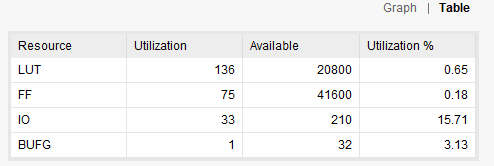
\includegraphics[width=0.7\textwidth]{image/2024-06-19-17-27-19.png}
    \caption{资源使用情况}
    \label{image_utilize_1}
\end{figure}
最终使用资源如图\ref{image_utilize_1}所示。
% 第三部分
\section*{\fourhao 三、仿真结果}
\xiaosihao
\setstretch{1.5}
% 对仿真图像要有解释,要对所有的可能性进行标注及解释
% 按照基础任务、提高任务和拓展任务分别给出仿真结果
\subsection*{基础任务}
\vspace{-0.6cm}
\begin{figure}[H]
    \centering
    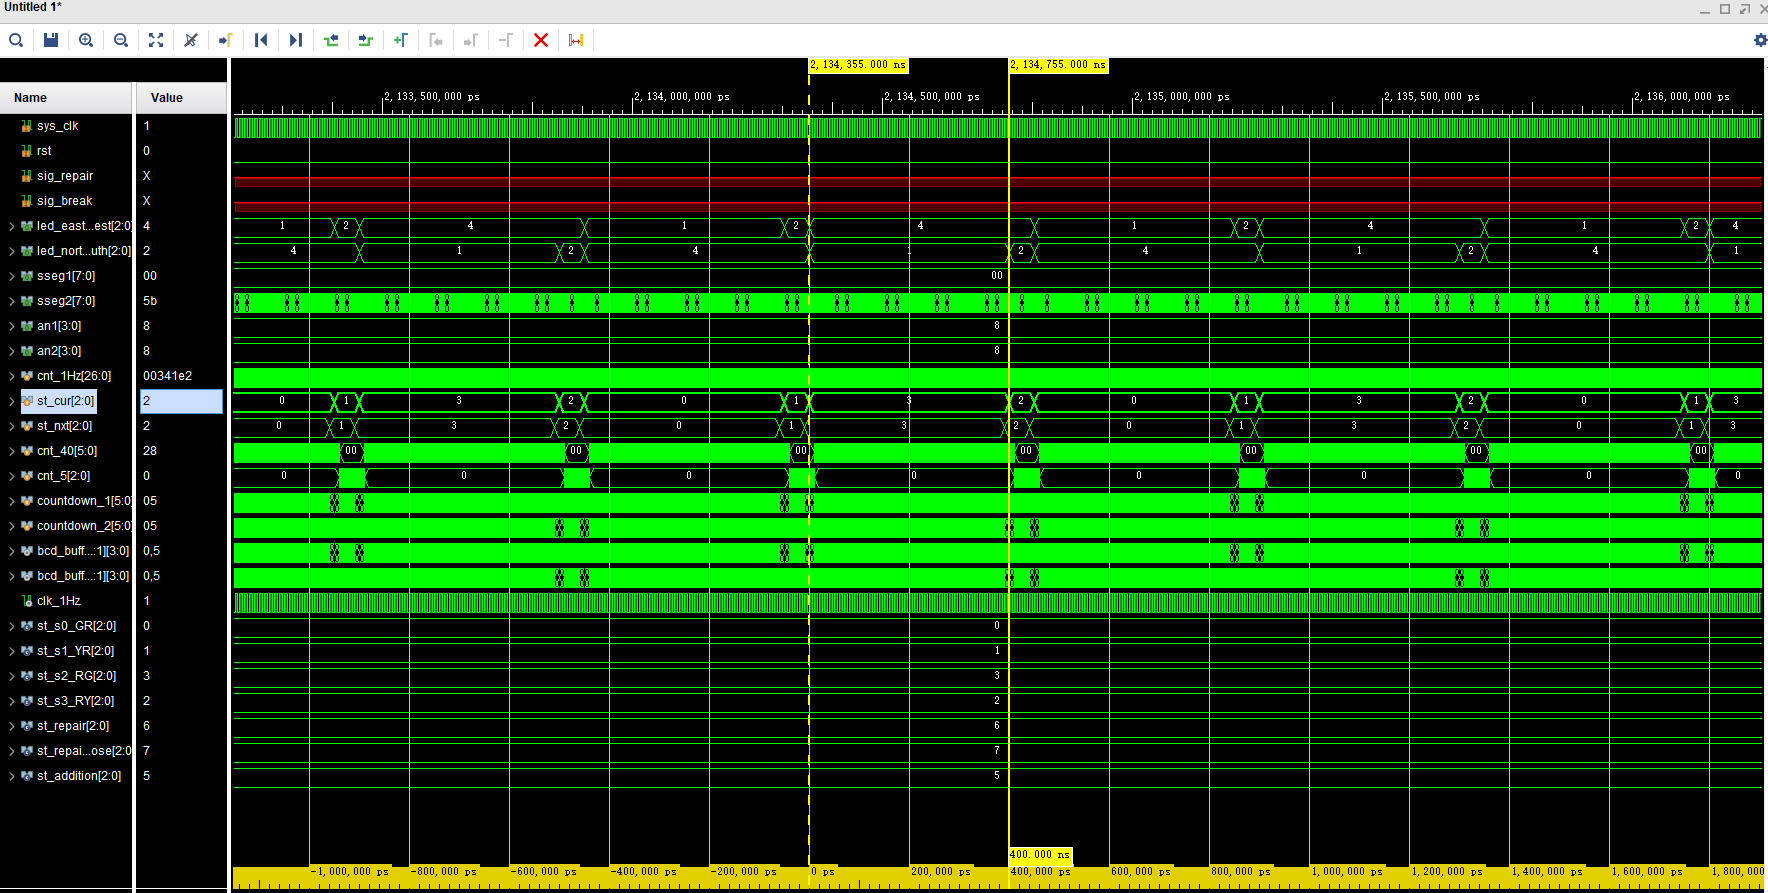
\includegraphics[width=0.7\textwidth]{image/2024-06-18-22-23-15.png}
    \caption{仿真结果1}
    \label{image_base_sim_1}
\end{figure}
\begin{figure}[H]
    \centering
    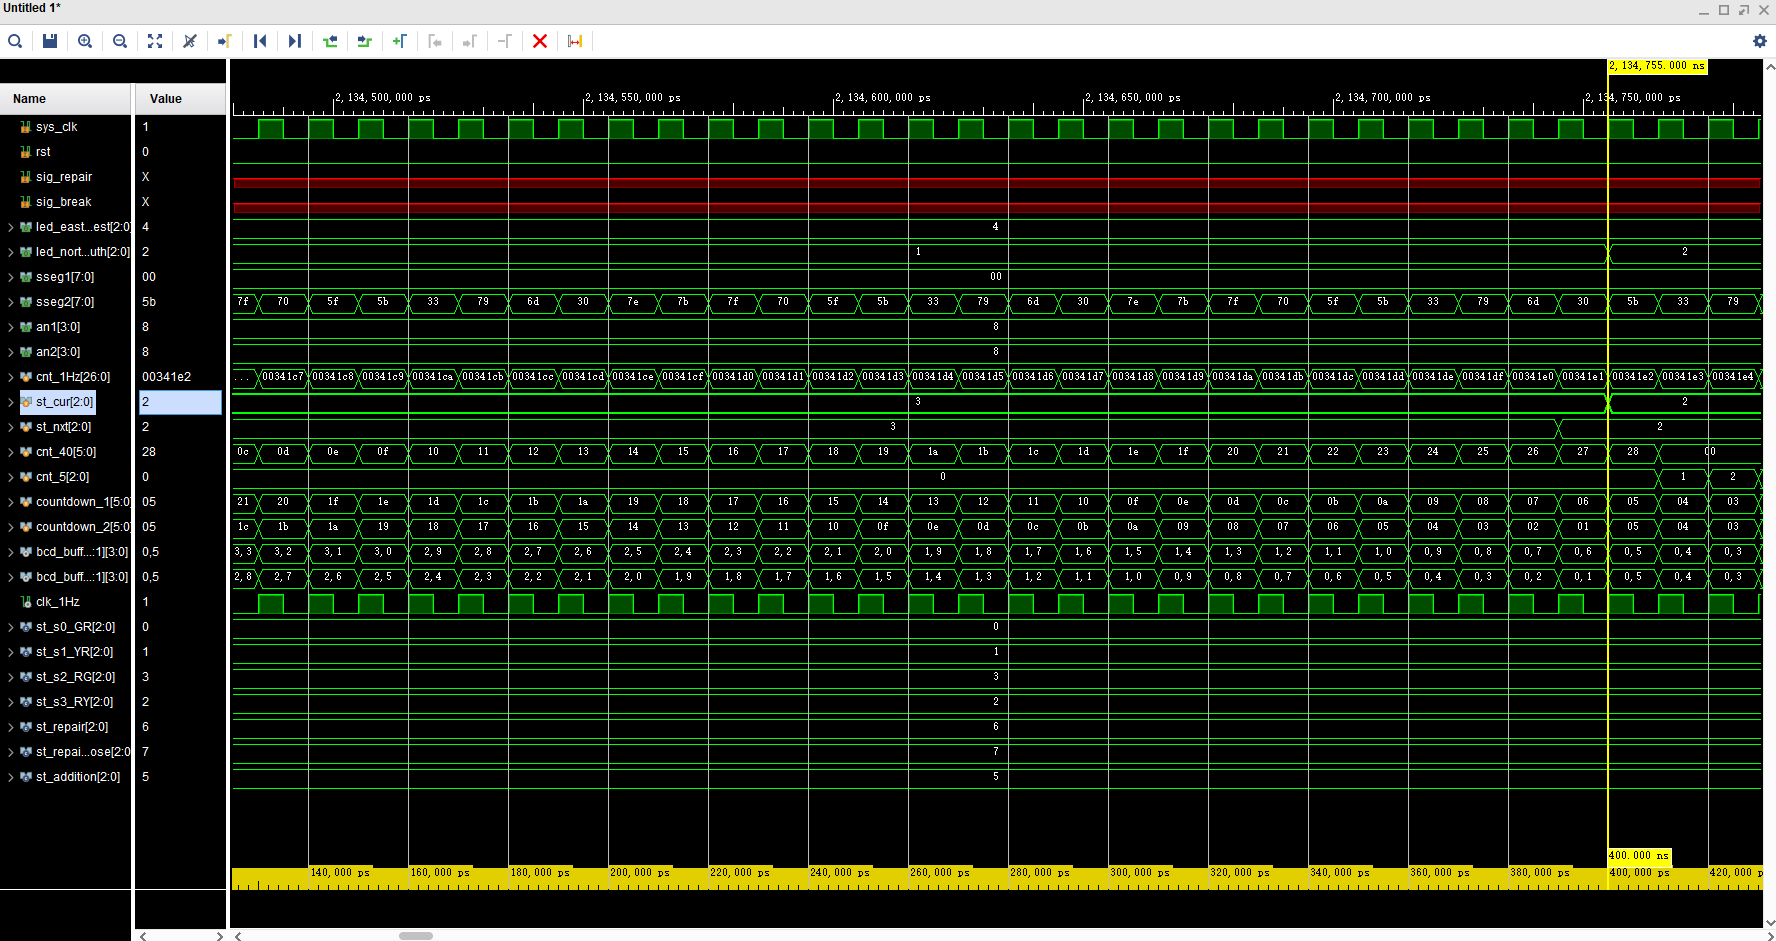
\includegraphics[width=0.7\textwidth]{image/2024-06-18-22-23-37.png}
    \caption{仿真结果2}
    \label{image_base_sim_2}
\end{figure}
具体的仿真结果见图\ref{image_base_sim_1}和图\ref{image_base_sim_2}所示, 为了便于仿真, 系统运行基准时钟选择100MHz, 
分析状态机工作过程, 满足基本设计要求的四个状态, 状态时间满足40s和5s的要求, 并通过组合逻辑电路实现交通灯控制信号的输出和倒计时, 倒计时也准确无误。
\subsection*{提高任务}
\begin{figure}[htbp]
    \centering
    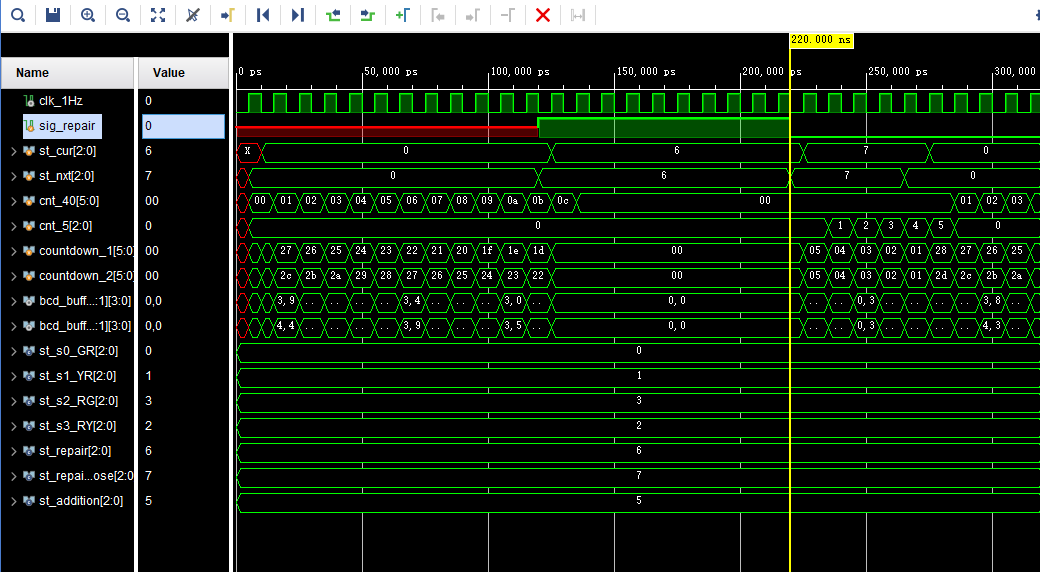
\includegraphics[width=0.7\textwidth]{image/2024-06-19-15-31-01.png}
    \caption{检修状态仿真结果}
    \label{image_repair_sim}
\end{figure}
提高任务中,添加检修状态的仿真结果见图\ref{image_repair_sim}, 当检测到检修信号为高电平时, 次态进入检修状态, 当检测到检修信号取消, 进入退出状态, 倒计时5s后进入s0状态。
\subsection*{拓展任务}
\begin{figure}[htbp]
    \centering
    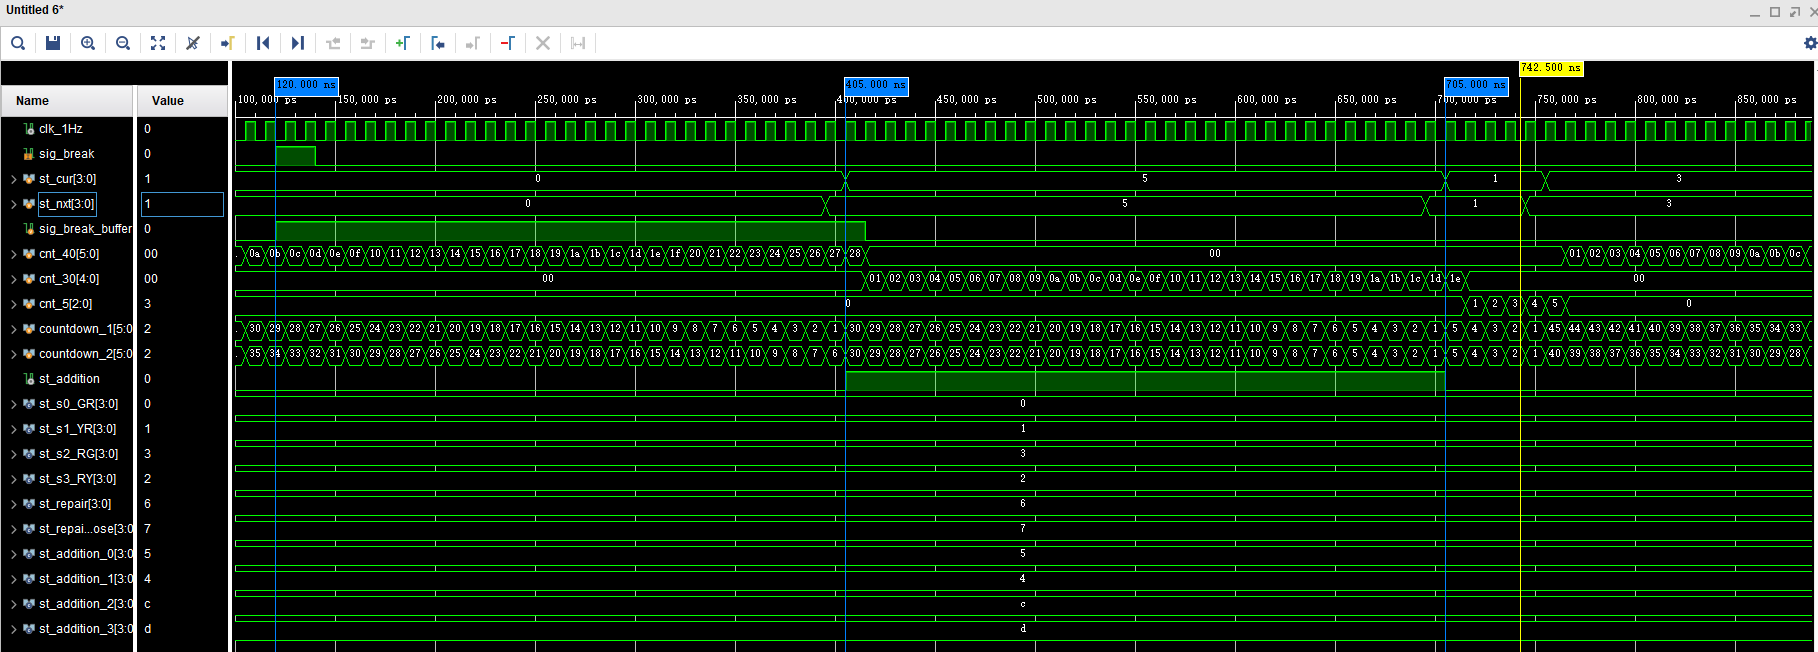
\includegraphics[width=0.7\textwidth]{image/2024-06-19-17-08-24.png}
    \caption{附加状态仿真结果}
    \label{image_addition_sim}
\end{figure}
拓展任务之中, 针对附加状态的仿真结果见图\ref{image_addition_sim}, 在该仿真结果中, 添加了三个Marker, 分别是该系统检测到输入的附加状态上升沿, 通过buffer缓存该输入信号, 当当前状态即将结束进入下一状态时, 系统进入附加状态0, 此时buffer自己清空, 之后经过30s的倒计时后, 系统按顺序进入刚才即将进入的状态st\_s1。
% 第四部分
\section*{\fourhao 四、硬件验证结果}
\xiaosihao
\setstretch{1.5}
% 记录加编程器与拨码开关和发光二极管、数码管等的连接情况。记录开发板硬件验证结果,并分析其结果的正确性。
% 按照基础任务、提高任务和拓展任务分别分析
\subsection*{基础任务}
\begin{figure}[htbp]
    \centering
    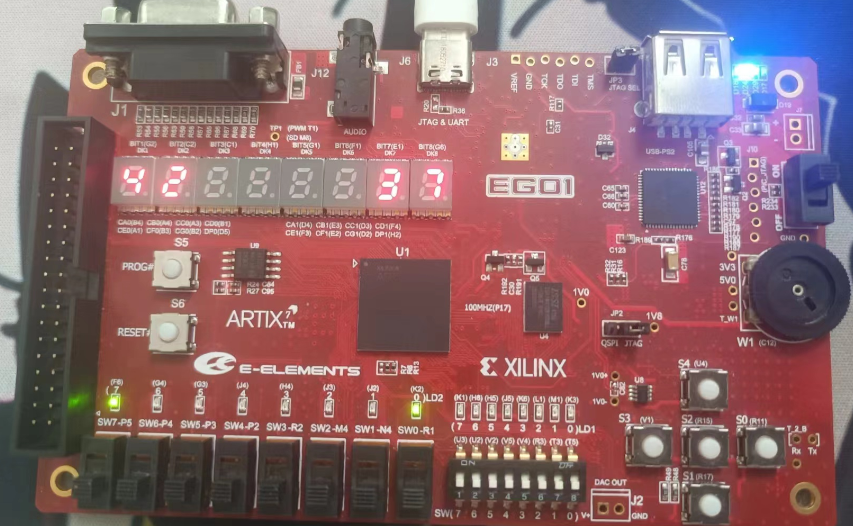
\includegraphics[width=0.5\textwidth]{image/2024-06-19-14-07-53.png}
    \caption{基础任务硬件验证结果}
    \label{image_base_verify}
\end{figure}
基础任务实现的硬件验证结果如图\ref{image_base_verify}所示, 左三LED和右三LED分别
作为东西方向和南北方向的红、黄和绿灯, 其上数码管显示的倒计时对应其时间。
\subsection*{提高任务}
\begin{figure}
    \begin{minipage}[t]{0.45\linewidth}
        \centering
        
\includegraphics[width=0.7\textwidth]{image/2024-06-19-20-58-40.png}
        \caption{检修状态}
        \label{image_repair_verify_1}
    \end{minipage}
    \begin{minipage}[t]{0.45\linewidth}
        \centering
        
\includegraphics[width=0.7\textwidth]{image/2024-06-19-21-00-32.png}
        \caption{检修退出状态}
        \label{image_repair_verify_2}
    \end{minipage}
\end{figure}
如图\ref{image_repair_verify_1}所示为系统进入检修状态, 左下角开关SW置1, 红绿灯全灭, 倒计时固定为00和00,
 图\ref{image_repair_verify_2}所示为开关SW7拨下, 系统进入退出检修状态, 倒计时5s之后进入s0状态。\\ 
\subsection*{拓展任务}
\begin{figure}[htbp]
    \centering
    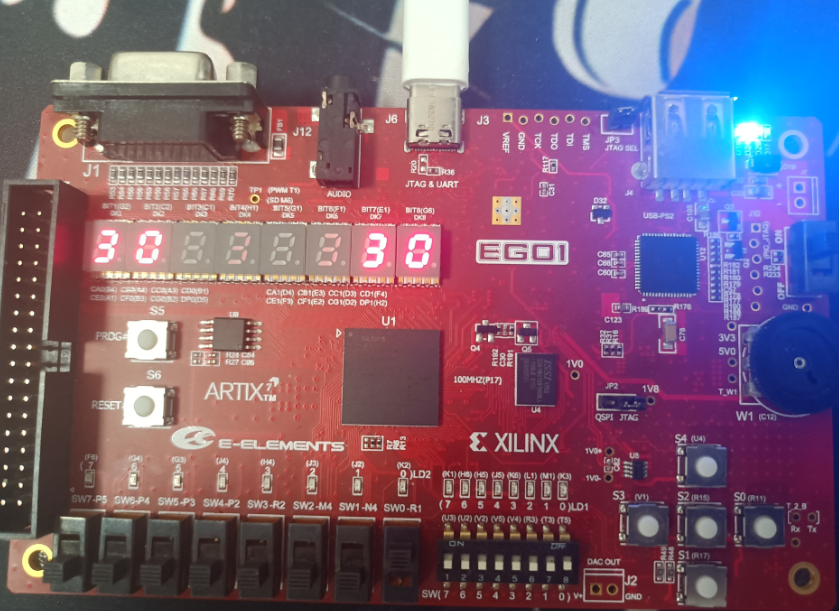
\includegraphics[width=0.5\textwidth]{image/2024-06-20-09-45-50.png}
    \caption{拓展任务硬件验证结果}
    \label{image_addition_verify}
\end{figure}
基础任务实现的硬件验证结果如图\ref{image_addition_verify}所示, 设置拨码开关后, 当前状态结束后进入附加模式,
 在附加模式下开始30s的倒计时, 同时红绿灯控制为全灭, 倒计时结束, 进入退出循环前的下一个状态。\\
% 第五部分
\section*{\fourhao 五、问题解决}
\xiaosihao
\setstretch{1.5}
% 设计过程中遇到的问题及解决的方法。
\subsection*{100MHz时钟的100M分频仿真时间过大}
开始的时候直接考虑了, 在仿真的时候改变该工作基准时钟, 采用系统时钟作为工作时钟, 观察状态机工作过程即可。但在仿真和综合间来回切换代码较为繁琐, 此时可以通过与C语言宏定义类似的方法实现代码的快速更改, 如下所示:
\begin{lstlisting}[language=Verilog, caption={编译指令应用}]
`ifdef STIMULATION
assign clk_1Hz = sys_clk;
`else
wire clk_1Hz;
/* 产生1.00117Hz信号 */
clk_div_32bit  clk_div_32bit_inst (
    .clk(sys_clk),
    .rstn(!rst),
    .step_freq(32'd43),
    .clk_out(clk_1Hz)
);
`endif
\end{lstlisting}
\subsection*{确认约束文件无误, 但布局布线时提示有端口sig\_break没有连接}
\begin{figure}[H]
    \centering
    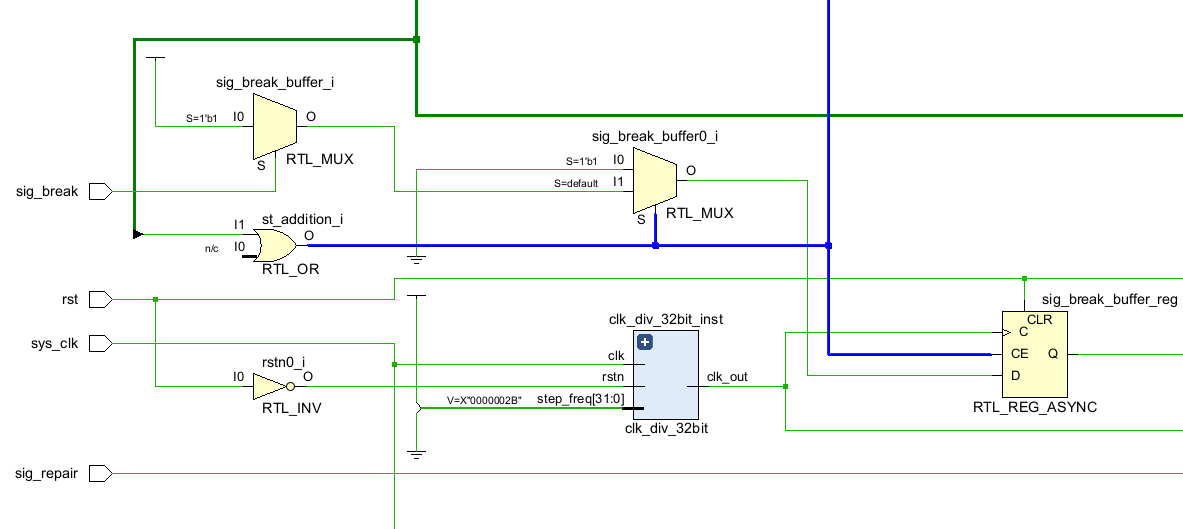
\includegraphics[width=0.7\textwidth]{image/2024-06-19-17-41-30.png}
    \caption{RTL原理图}
    \label{image_QA_1}
\end{figure}
\begin{figure}[htbp]
    \centering
    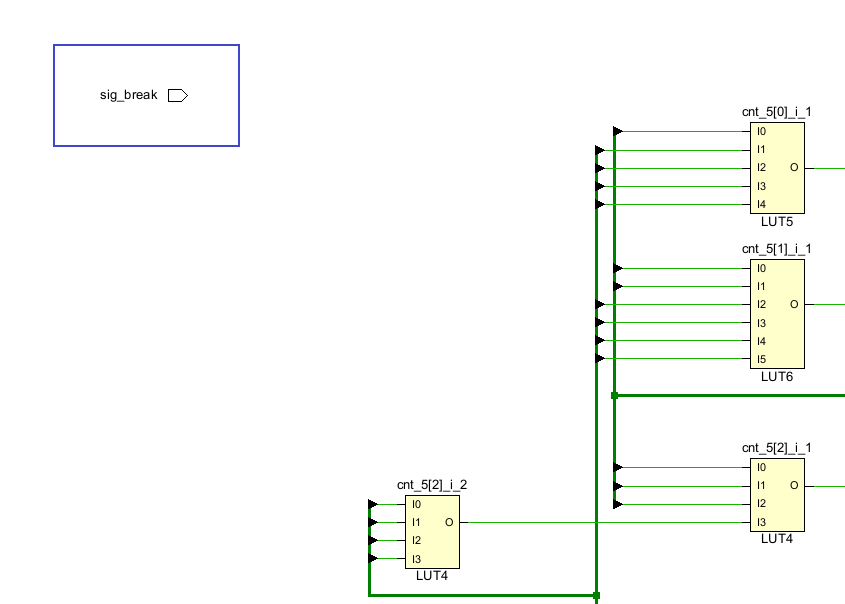
\includegraphics[width=0.5\textwidth]{image/2024-06-19-17-44-00.png}
    \caption{综合结果}
    \label{image_QA_2}
\end{figure}
针对该报错检查RTL分析原理图\ref{image_QA_1}, 确定在进行描述时无误, 再检查综合结果, 综合结果见图\ref{image_QA_2}, 
可以看到在RTL中设计无误的sig信号被综合工具优化掉, 该端口没有连接任何信息。检查Warning信息, 可以看到如下Warning\\
\begin{lstlisting}[language=Verilog]
[Synth 8-7129] Port sig_break in module traffic\_light is either unconnected or has no load
\end{lstlisting}
通过对综合结果的分析, 最终将问题锁定到对sig\_break信号的缓存模块, sig\_break信号作为该时序逻辑中if的判断条件的同时,
 作为了时序逻辑的边沿触发条件, 相同的应用有rst接口, 但是通过综合结果可以看到, 综合工具对rst信号有单独的处理, 同样是
 使触发器清零, st\_addition就是通过赋值的方式清零, 但是rst信号是直接连接到了触发器的复位端上, 所以sig\_break信号无
 法像rst一样, 即在敏感列表又在条件判断, 综合工具认为其没有被使用而将其优化掉了。\\
 \newpage
 错误代码如下:
\begin{lstlisting}[language=Verilog, caption={综合不理想代码}]
/* 附加模式缓存 */
reg sig_break_buffer;
always @(posedge clk_1Hz or posedge rst or posedge sig_break) begin
    if (rst == 1'b1 || st_addition == 1'b1) begin
        sig_break_buffer <= 1'b0;
    end
    else if (sig_break == 1'b1) begin
        sig_break_buffer <= 1'b1;
    end
    else begin
        sig_break_buffer <= sig_break_buffer;
    end
end
\end{lstlisting}
\subsection*{写状态机过程中出现仿真正确但硬件验证结果混乱, 无规律可循}
当输出无规律可循时, 一般是由于综合的过程中产生了锁存器(latch), latch的输入状态可能多次变化,容易产生毛刺,为整个电路带来严重的不确定性。
除非设计需求, 在设计时应该极力避免latch的产生。\\
在初次发现问题时, 一直进行的行为仿真和时序仿真的仿真结果无误, 但是硬件验证结果与仿真结果严重偏移, 通过ILA核进行板上调试会发现数据错误, 但毫无规律可循。
该问题无法明确找到对应的解决方案, 因此到图书馆查阅更多资料进行系统性学习, 偶然在《Verilog传奇--从电路出发的HDL代码设计》一书中看到专门针对latch危害的讨论, 在理解其危害后自检代码发现问题, 
问题出现在三段状态机中求解下一个状态的\textbf{组合逻辑电路}中, 由于条件判断的if-else结构不完整, 导致Vivado综合出了latch, 直接导致状态机的状态混乱。\\
进一步查阅资料, 这种情况仅发生在组合逻辑电路中, 当组合逻辑中的条件分支语句不完整(不收敛)一般会综合产生latch, 而时序逻辑中的变量, 其本身就具有存储功能, 所以不会产生该问题。\\
在了解了以上内容后, 再回到Vivado之中, 甚至可以看到综合工具会进行Warning提醒: "综合产生了一个latch。"\\
会综合产生latch的几种情况(组合逻辑):if-else结构不完整、case结构不完整、信号幅值的等号右侧有其本身、always块的敏感列表没有列全。\\
本质上, 综合产生latch是因为综合工具判断该组合逻辑需要存储功能, 如if-else结构不完整的话, 综合工具默认缺省的else的分支下待赋值的信号值不变, 信号不变就意味着需要存储单元, 导致其被综合成latch结构。
% 第六部分
\section*{\fourhao 六、心得体会}
\xiaosihao
\setstretch{1.5}
通过对三层任务分级, 基本掌握简单的三段式状态机设计。本次设计中最重要的收获是养成了一种思维习惯, 以往在进行通用计算机或者MCU
上的程序设计时, 是以一种串行执行的思路, 通过堆砌条件控制语句、中断控制、多线程等方式实现复杂的系统, 而在FPGA的硬件设计中, 
主要是通过FSM去实现复杂的系统, 在进行交通灯控制器的设计过程中, 逐渐在学会如何以不同状态看待一个复杂系统的实现, 将一个复杂
的任务分解为FSM的不同状态和不同输出。\\
同时也深刻的体会到FPGA技术的优越性, 数电课程中设计一个基础任务就要经过反复的化简、建模和绘制时序图, 但在Verilog语
言的帮助下, 通过成熟的三段式FSM描述方法, 不仅可以快速的实现一个FSM, 还可以保证其稳定性, 并且直接进行时序仿真可以
高效的从时序图中发现时序逻辑电路的问题。
\end{document}
